%% \documentclass[handout,t]{beamer} % HANDOUT
\documentclass[handout,notes=show,t]{beamer} % NOTES
%% \documentclass[t]{beamer} % SLIDES

\usetheme{SIGIL}
\usepackage{beamer-tools-sigil}

%%
%%  INCLUDE: math.tex
%%  
%%  basic mathematical symbols and constructs (not specific to cooccurrences)
%%


%% \setN, \setN[0], \setZ, \setQ, \setR, \setC
%% abbreviations for common number spaces
\newcommand{\setN}[1][]{\mathbb{N}_{#1}} % allows \setN and \setN[0]
\newcommand{\setZ}{\mathbb{Z}}
\newcommand{\setQ}{\mathbb{Q}}
\newcommand{\setR}{\mathbb{R}}
\newcommand{\setC}{\mathbb{C}}

%% \set{el_1, el_2, ...};  \setdef{el}{condition};  \bigset{..}, \bigsetdef{..}{..}
%% extensional and intensional definition of sets, with "big" versions (like \bigl etc.)
\newcommand{\set}[1]{\left\{#1\right\}}
\newcommand{\setdef}[2]{\set{#1\,\left|\,#2\right.}}
\newcommand{\bigset}[1]{\bigl\{#1\bigr\}}
\newcommand{\bigsetdef}[2]{\bigset{#1\bigm|#2}}
\newcommand{\Bigset}[1]{\Bigl\{#1\Bigr\}}
\newcommand{\Bigsetdef}[2]{\Bigset{#1\Bigm|#2}}
\newcommand{\biggset}[1]{\biggl\{#1\biggr\}}
\newcommand{\biggsetdef}[2]{\biggset{#1\biggm|#2}}

%% \compl{X} = complement of set X
\newcommand{\compl}[1]{\mathcal{C} #1}

%% \eps == \epsilon, \si == \sigma, \sisi == \sigma^2, \ka == \kappa
\newcommand{\eps}{\epsilon}
\newcommand{\si}{\sigma}
\newcommand{\sisi}{\sigma^2}
\newcommand{\ka}{\kappa}

%% \abs{expr}, \bigabs{expr}, \norm{expr}, \bignorm{expr}
%% absolute value and norm of expression, with "big" versions
\newcommand{\abs}[1]{\left\lvert#1\right\rvert}
\newcommand{\bigabs}[1]{\bigl\lvert#1\bigr\rvert}
\newcommand{\norm}[1]{\left\lVert#1\right\rVert}
\newcommand{\bignorm}[1]{\bigl\lVert#1\bigr\rVert}

%% \constpi == constant PI (in bold font)
\newcommand{\constpi}{\boldsymbol{\pi}}

%% \dx == "dx";  \dx[z] == "dz";  \dpi == \dx[\pi];  
%% \dG == \dx[G], \dt == \dx[t]
\newcommand{\dx}[1][x]{\,d#1}
\newcommand{\dpi}{\dx[\pi]}
\newcommand{\dG}{\dx[G]}
\newcommand{\dt}{\dx[t]}

%% \Int{\frac{1}{2} x^2}_a^b
%% anti-derivative evaluated to compute definite integral
\newcommand{\Int}[1]{\left[#1\right]}

%% \limdownto{x}{0}
%% limit from above for x -> 0
\newcommand{\limdownto}[2]{\lim_{#1\,\downarrow\,#2}}

%% \iffdef == ":<=>";  \iffdefR == "<=>:"
\newcommand{\iffdef}{\;:\!\iff}
\newcommand{\iffdefR}{\iff\!:\;}

%% \logten(x) 
%% base 10 logarithm, which is always used in the UCS system
\newcommand{\logten}{\log_{10}}

%% \e+3, \e-6, \e-{12}, 5.5\x\e-3
%% engineering-style notation (orders of magnitude) for floating-point numbers
\newcommand{\e}[2]{10^{\ifthenelse{\equal{#1}{+}}{}{#1}#2}}
\newcommand{\x}{\cdot}

%% \Landau{ n^2 }, \bigLandau{ N^2 }
%% Landau symbol ("big oh notation")
\newcommand{\Landau}[1]{\mathcal{O}\left({#1}\right)}
\newcommand{\bigLandau}[1]{\mathcal{O}\bigl({#1}\bigr)}


%%% Local Variables: 
%%% mode: latex
%%% TeX-master: t
%%% End: 
  % basic mathematical notation
%%
%%  INCLUDE: stat.tex
%%  
%%  symbols and notation for probability theory and statistics
%%


%% \p{X=k};  \pC{X=k}{Y=l};  \pscale{\frac{Z}{S^2}}
%% probability P(X=k), conditional probability P(X=k|Y=l), and variants with scaled parentheses
\newcommand{\p}[1]{\mathop{\mathrm{Pr}}\bigl(#1\bigr)}
\newcommand{\pscale}[1]{\mathop{\mathrm{Pr}}\left(#1\right)}
\newcommand{\pC}[2]{\p{#1\bigm|#2}} 
\newcommand{\pCscale}[2]{\pscale{#1\,\left|\,#2\right.}} 

%% \Exp{X};  \Var{X};  \Exp[0]{X};  \Var[0]{X};  \Expscale{X};  \Varscale{X}
%% expectation E[X] and variance V[X], expectation and variance under null hypothesis, 
%% and variants with scaled brackets
\newcommand{\Exp}[2][]{E_{#1}\bigl[#2\bigr]}
\newcommand{\Var}[2][]{\mathop{\mathrm{Var}}_{#1}\bigl[#2\bigr]}
\newcommand{\Expscale}[2][]{E_{#1}\left[#2\right]}
\newcommand{\Varscale}[2][]{\mathop{\mathrm{Var}}_{#1}\left[#2\right]}

%% \I{f_i = M};  \bigI{\sum_{i=1}^S f_i = N}
%% indicator variable (as in Baayen 2001), and variant with explicitly scaled brackets
\newcommand{\I}[1]{I_{\left[#1\right]}}
\newcommand{\bigI}[1]{I_{\bigl[#1\bigr]}}

%% \Hind;  \Hhom;  \Hnull{\kappa = x}
%% null hypothesis of independence and homogeneity; general null hypothesis identified by condition
\newcommand{\Hind}{H_0}
\newcommand{\Hhom}{H_{0,\, hom}}
\newcommand{\Hnull}[1]{H_{#1}}

%% \confint{\kappa};  \confint[0.99]{\kappa}
%% confidence interval for specified population characteristic (conf. level defaults to \alpha)
\newcommand{\confint}[2][\alpha]{I_{#2,\,#1}}

%% \df = 1
%% degrees of freedom
\newcommand{\df}{\mathit{df}}


%%% Local Variables: 
%%% mode: latex
%%% TeX-master: t
%%% End: 
  % notation for probability theory and statistics
%%
%% convenience macros for linear algebra (vectors and matrices)
%%

%% \Vector[i]{x} ... vector variable with optional _superscript_ index in parentheses
%% \Vector[']{x} ... special case: ' superscript not enclosed in parentheses
%% \vx, \vy, \vz ... abbreviations for common vector names
\newcommand{\Vector}[2][]{\mathbf{#2}\ifthenelse{\equal{#1}{}}{}{^{(#1)}}}
\newcommand{\vx}[1][]{\Vector[#1]{x}}
\newcommand{\vy}[1][]{\Vector[#1]{y}}
\newcommand{\vz}[1][]{\Vector[#1]{z}}
\newcommand{\vu}[1][]{\Vector[#1]{u}}
\newcommand{\vv}[1][]{\Vector[#1]{v}}
\newcommand{\vw}[1][]{\Vector[#1]{w}}
\newcommand{\vm}[1][]{\Vector[#1]{m}} 
\newcommand{\va}[1][]{\Vector[#1]{a}} % vectors of coefficients
\newcommand{\vb}[1][]{\Vector[#1]{b}} % for basis
\newcommand{\ve}[1][]{\Vector[#1]{e}} % for standard basis of R^n
\newcommand{\vn}[1][]{\Vector[#1]{n}} % normal vector
\newcommand{\vnull}[1][]{\Vector[#1]{0}} % neutral element

%% \Span{\vb[1],\ldots,\vb[k]} ... span of set of vectors
%% \Rank{...} ... rank of set of vectors or matrix
%% \Det{...}, \det A ... determinant of a set of vectors / a matrix A
%% \Image{f}, \Kernel{f} ... image and kernel of a linear map
\newcommand{\Span}[1]{\mathop{\text{sp}}\left(#1\right)}
\newcommand{\Rank}[1]{\mathop{\text{rank}}\left(#1\right)}
\newcommand{\Det}[1]{\mathop{\text{Det}}\left(#1\right)}
%% \det is already defined in the standard library
\newcommand{\Image}[1]{\mathop{\text{Im}}\left(#1\right)}
\newcommand{\Kernel}[1]{\mathop{\text{Ker}}\left(#1\right)}

%% \dist[2]{\vx}{\vy} ... distance between two vectors (p-metric)
\newcommand{\dist}[3][]{d_{#1}\left(#2, #3\right)}
\newcommand{\bigdist}[3][]{d_{#1}\bigl(#2, #3\bigr)}

%% \sprod{\vu}{\vv} ... scalar product
\newcommand{\sprod}[2]{\left\langle #1, #2 \right\rangle}
\newcommand{\bigsprod}[2]{\bigl\langle #1, #2 \bigr\rangle}


%%% Local Variables: 
%%% mode: latex
%%% TeX-master: ""
%%% End: 
% convenience macros for vectors and matrices

%%%
%%% local configuration adjustments
%%%

%%% You can change pre-defined colours here, override built-in macros from the
%%% style definition and standard library, as well as define macros needed by
%%% all local documents.

%%% e.g. adjust counterpoint (dark green) for data projectors where greens are
%%% far too bright, as well as green component of light colour and pure green
%%% (of course, it's a better solution to adjust the gamma settings of your monitor)
%%
%% \definecolor{counterpoint}{rgb}{.1, .3, 0}
%% \definecolor{light}{rgb}{.45, .3, .55}
%% \definecolor{puregreen}{rgb}{0, .35, 0}

%% ----- extra packages we need to load

\usepackage{tikz}
\usepackage{alltt}              % code examples with nicely formatted comments
\usepackage{rotating}


%% ----- author and copyright messages (so updates are automatically inserted into all files)
\newcommand{\sigilauthors}{%
  \author[SIGIL]{Designed by Stefan Evert\inst{1} and Marco Baroni\inst{2}}
  \institute[Evert \& Baroni]{
    \inst{1}Computational Corpus Linguistics Group\\
    Friedrich-Alexander-Universit�t Erlangen-N�rnberg, Germany
    \and
    \inst{2}Center for Mind/Brain Sciences (CIMeC)\\
    University of Trento, Italy
  }
}
\newcommand{\sigilcopyright}{%
  \date[sigil.r-forge.r-project.org]{%
    \primary{\footnotesize\url{http://SIGIL.r-forge.r-project.org/}}\\
    \light{\tiny Copyright \textcopyright\ 2007--2018 Evert \& Baroni}}
}

%% ----- automatically show TOC reminder at beginning of each subsection
\AtBeginSubsection[]
{
  \begin{frame}
    \frametitle{Outline}
    \tableofcontents[current,currentsubsection]
  \end{frame}
}

%% ----- some useful macros for the SIGIL course

\newenvironment{Rcode}[1][]{%
  \setbeamercolor{block title}{fg=counterpoint,bg=counterpoint!15!white}%
  \setbeamercolor{block body}{bg=counterpoint!5!white}\small%
  \begin{block}{#1}\begin{alltt}\ungap[1]}{%
      \ungap[1]\end{alltt}\end{block}} % \end{alltt} ... to deconfuse emacs

%% use \sbox{\Rbox} ... \usebox{\Rbox} to insert arbitray latex into Rcode environment
\newsavebox{\Rbox}

%% > plot(x,y)      \REM{this produces a scatterplot}
\newcommand{\REM}[2][\small]{\textsf{#1\color{primary}\# #2}}

%% nice colour for R output: \begin{Rout} .. \end{Rout}
\newenvironment{Rout}[1][\footnotesize]{%
  \begin{footnotesize}#1\color{secondary}\bfseries}{%
    \color{black}\mdseries\end{footnotesize}}

%% rotated column labels for table (to fit long text into narrow columns
\newcommand{\rotLabel}[2][60]{\begin{rotate}{#1}#2\end{rotate}}
 % local adjustments to configuration and macros

%%%%%%%%%%%%%%%%%%%%%%%%%%%%%%%%%%%%%%%%%%%%%%%%%%%%%%%%%%%%%%%%%%%%%%
%% Titlepage

\title[1.\ Introduction]{Statistical Inference: a Gentle Introduction
  for Linguists and similar creatures (SIGIL)}
\subtitle{With practical examples in GNU R}
\sigilauthors
\sigilcopyright

\begin{document}

\frame{\titlepage}

%%%%%%%%%%%%%%%%%%%%%%%%%%%%%%%%%%%%%%%%%%%%%%%%%%%%%%%%%%%%%%%%%%%%%%

\section*{Outline}
\frame{ 
  \frametitle{Outline}
  \tableofcontents
}

%%%%%%%%%%%%%%%%%%%%%%%%%%%%%%%%%%%%%%%%%%%%%%%%%%%%%%%%%%%%%%%%%%%%%%
\section{General Introduction}

%%%%%%%%%%%%%%%%%%%%%%%%%%%%%%%%%%%%%%%%%%
\subsection{Statistical inference and GNU R}

\begin{frame}
  \frametitle{Why do we need statistics?}

  \begin{itemize}
  \item<2-> \h{Significance} (control for sampling variation)
    \begin{itemize}
    \item all linguistic data are samples (of language, speakers, \ldots)
    \item observed effects may be coincidence of particular sample
    \item[\So] \textbf{inferential statistics}
    \item[]
    \end{itemize}
  \item<3-> Managing \h{large data sets}
    \begin{itemize}
    \item statistical summaries, data analysis, visualisation
    \item e.g.\ collocations as compact summary of word usage
    \item[\So] \textbf{descriptive statistics}
    \item[]
    \end{itemize}
  \item<4-> Discovering \h{latent} (hidden) \h{properties}
    \begin{itemize}
    \item clustering, multivariate analysis, distributional semantics
    \item advanced statistical modelling (e.g.\ mixed-effects models)
    \item[\So] \textbf{exploratory data analysis}
    \end{itemize}
  \end{itemize}
\end{frame}

\begin{frame}
  \frametitle{What everyone needs to know about statistics}

  \begin{itemize}
  \item<2-> Population \vs sample
  \item<3-> Random variables \& scales of measurement
  \item<4-> Basic principles of statistical inference
  \item<5-> Statistical tests: null hypothesis, p-value, assumptions
  \item<6-> Significance \vs effect size (relevance)
  \item<7-> Estimation: MLE, confidence interval
  \item<8-> Statistical modelling (regression, general linear model, \ldots)
  \item<9-> Applicability and limitations of statistical methods
  \item<10->[\hand] Gain practical experience with statistical software
  \end{itemize}

  \gap\onslide<11->
  What you can do on your own:
  \begin{itemize}
  \item Learn about specific statistical tests and procedures
  \end{itemize}
\end{frame}

\begin{frame}
  \frametitle{\textbf{R} -- An environment for statistical programming}

  \begin{itemize}
  \item<1-> ``Traditional'' statistical software packages offer specialised
    procedures (e.g.\ SAS) or interactive GUI (e.g.\ SPSS)
    \begin{itemize}
    \item[]
    \end{itemize}
  \item<2-> New approach: statistical programming language \hh{S} with interactive
    environment (Bell Labs, since 1976)
    \begin{itemize}
    \item \emph{White Book} (version 3, 1992); \emph{Green Book} (version
      4, 1998)
    \item commercial: S-Plus (Insightful Corporation, since 1987)
    \item[]
    \end{itemize}
  \item<3-> \hh{R} is an open-source implementation of the S language
    \begin{itemize}
    \item originally by Ross Ihaka and Robert Gentleman (Auckland)
    \item open-source development since mid-1997
    \end{itemize}
  \end{itemize}
\end{frame}

\begin{frame}
  \frametitle{\textbf{R} -- An environment for statistical programming}
  
  \vspace{5mm}
  \begin{columns}[c]
    \begin{column}{35mm}
      
\includegraphics[width=4cm]{img/Rlogo}
    \end{column}
    \begin{column}{7cm}
      \begin{itemize}
      \item binary packages available for Linux, Mac OS X and Windows
      \item 64-bit support for large data sets
      \item extensive documentation \& tutorials
      \item thousands of add-on packages ready to install from CRAN
      \end{itemize}
    \end{column}
  \end{columns}
  \vspace{8mm}
  \begin{center}
    \hh{\large\url{http://www.R-project.org/}}
    
    \vspace{6mm}
    Recommended cross-platform GUI:\\
    \h{RStudio} from \url{http://www.rstudio.com/ide/}
  \end{center}
\end{frame}

\begin{frame}
  \frametitle{More about \textbf{R}}
  
  \begin{itemize}
  \item Advantages of R
    \begin{itemize}
    \item free \& open source
    \item many add-on packages with state-of-the-art algorithms
    \item large, enthusiastic and helpful user community
    \item easy to automate and extend (every analysis is a program)
    \item no point \& click interface
    \item[]
    \end{itemize}
  \item<2-> Disadvantages
    \begin{itemize}
    \item learning curve sometimes rather steep
    \item not very good at manipulating non-English text
    \item no built-in data editor (spreadsheet)
    \item no point \& click interface
    \end{itemize}
  \end{itemize}
\end{frame}

%%%%%%%%%%%%%%%%%%%%%%%%%%%%%%%%%%%%%%%%%%
\subsection{About this course}

\begin{frame}
  \frametitle{Goals of the course}

  \begin{itemize}
  \item Basic principles of statistical inference
  \item Elementary hypothesis tests, estimators \& models
  \item Hands-on work with R on real-life data sets
  \item Data manipulation and basic R programming skills
  \item Get to know R implementations of statistical techniques,\\
    data analysis and visualisation methods that are useful in various areas
    of (computational) linguistics along the way
  \end{itemize}

  \pause\gap
  What this course is \emph{\primary{not}} about:
  \begin{itemize}
  \item Deeper mathematical foundations of statistics
  \item Specific (advanced) statistical methods
  \item Cookbook recipes for particular analyses with R
  \end{itemize}

\end{frame}

{
\newcommand{\halfday}{\primary{\textsc{(h)}}}
\newcommand{\fullday}{\primary{\textsc{(f)}}}
\begin{frame}
  \frametitle{Course units}
  
  \begin{enumerate}
  \item R Basics: installation, data manipulation, input/output \halfday
  \item Corpus frequency data \& statistical inference \halfday
  \item Descriptive and inferential statistics for continuous data \fullday
  \item Co-occurrence, contingency tables and collocations \fullday\\
    + vectorised data processing, high-quality graphs
  \item Word frequency distributions with the \texttt{zipfR} package \halfday
  \item Regression and linear models \fullday
  \item Exploratory data analysis: clustering, visualisation, ML \halfday
  \item The non-randomness of corpus data: a GLM  approach \halfday
  \item Inter-annotator agreement \halfday
  \end{enumerate}

  \gap
  \halfday\ = half-day session / \fullday\ = full-day session (optimistic)
\end{frame}
}

\begin{frame}<beamer:1| handout:0>
  \frametitle{Introductions}

  \begin{center}
    
\includegraphics[height=5cm]{img/uncle-sam-wants-you}

    \vspace{5mm}
    \begin{Large}
      \h{Who are you?}
    \end{Large}
  \end{center}
\end{frame}

\begin{frame}
  \frametitle{Recommended textbooks: introductory level}

  \begin{itemize}
  \item Baroni, Marco \& Evert, Stefan (2008).  \primary{Statistical methods
      for corpus exploitation}.  In A.~L{\"u}deling \& M.~Kyt{\"o}
    (eds.), {\em Corpus Linguistics. An International Handbook}, Mouton de Gruyter.
    \begin{itemize}
    \item[]
    \end{itemize}
  \item Gries, Stefan~Th. (2013). \primary{\em Statistics for Linguistics with
      R: A Practical Introduction}, 2nd ed. Mouton de Gruyter. %
    \secondary{[\texteuro 29]}
    \begin{itemize}
    \item German original from Vandenhoek \& Ruprecht \secondary{[\texteuro 25]}
    \item[]
    \end{itemize}
  \item Johnson, Keith (2008). \primary{\em Quantitative Methods in Linguistics}.
    Blackwell. \secondary{[\texteuro 38]}
    \begin{itemize}
    \item[]
    \end{itemize}
  \item Peter Dalgaard (2008). \primary{\em Introductory Statistics with R},
     2nd ed. Springer. \secondary{[\texteuro 52]}
    \begin{itemize}
    \item[]
    \end{itemize}
  \end{itemize}
\end{frame}

\begin{frame}
  \frametitle{Recommended textbooks: advanced level}

  \begin{itemize}
  \item R.~Harald Baayen (2008). \primary{\emph{Analyzing Linguistic Data: A practical
        introduction to statistics}}. CUP. \secondary{[\texteuro 29]}
    \begin{itemize}
    \item \secondary{\footnotesize \href{http://www.sfs.uni-tuebingen.de/~hbaayen/publications/baayenCUPstats.pdf}{http://www.sfs.uni-tuebingen.de/\textasciitilde{}hbaayen/publications/}}
    \item[]
    \end{itemize}
  \item Morris H.\ DeGroot and Mark J.\ Schervish (2002). \primary{\emph{Probability and
      Statistics}}, 4th ed. Pearson Education Ltd. \secondary{[\texteuro 74]}
    \begin{itemize}
    \item[]
    \end{itemize}
  \item John M.\ Chambers (2008). \primary{\emph{Software for Data Analysis:
        Programming with R}}. Springer. \secondary{[\texteuro 85]}
    \begin{itemize}
    \item[]
    \end{itemize}
  \item Christopher Butler (1985), \primary{\emph{Statistics in Linguistics}}. Blackwell.
    \begin{itemize}
    \item out of print and available online for free download from
      \secondary{\scriptsize 
        \href{http://www.uwe.ac.uk/hlss/llas/statistics-in-linguistics/bkindex.shtml}{http://www.uwe.ac.uk/hlss/llas/statistics-in-linguistics/bkindex.shtml}}
    \item[]
    \end{itemize}
  \end{itemize}
\end{frame}

\begin{frame}
  \frametitle{Course materials}

  \begin{itemize}
  \item Handouts, example scripts and data sets are available on our homepage
    for this course:\\[4mm]
    \begin{center}
      \hh{\large\url{http://SIGIL.R-Forge.R-Project.org/}}
    \end{center}
    \gap[.5]
    (includes additional material, software, links, etc.)
  \end{itemize}

  \gap[3]
  Another interesting online course:
  \begin{itemize}
  \item Shravan Vasishth (2006--2009). \primary{\emph{The foundations of statistics: A
        simulation-based approach}}.
    \begin{itemize}
    \item \secondary{\footnotesize 
        \href{http://www.ling.uni-potsdam.de/~vasishth/SFLS.html}{http://www.ling.uni-potsdam.de/\textasciitilde{}vasishth/SFLS.html}}
    \end{itemize}
  \end{itemize}
\end{frame}

%%%%%%%%%%%%%%%%%%%%%%%%%%%%%%%%%%%%%%%%%%%%%%%%%%%%%%%%%%%%%%%%%%%%%%
\section{Getting Started With R}

%%%%%%%%%%%%%%%%%%%%%%%%%%%%%%%%%%%%%%%%%%
\subsection{Installation tips}

\begin{frame}
  \frametitle{Installation guide for Linux \& Mac OS X}

  \hh{Mac OS X}
  \begin{itemize}
  \item Download binary installer from \url{http://www.R-project.org/}
  \item Start GUI application \primary{\texttt{R}} (64-bit)
  \item Alternative: run from \primary{TextMate} or various other text editors
  \item Shell commmand \texttt{R} available for command-line use
  \end{itemize}

  \gap
  \hh{Linux} (Ubuntu and other popular distributions)
  \begin{itemize}
  \item Install R with standard package manager (e.g.\ \emph{Synaptic})
  \item Add CRAN repository to obtain up-to-date version of R
    \begin{itemize}
    \item e.g.\ \secondary{http://cran.at.r-project.org/bin/linux/ubuntu precise/}
    \item pkgs: \counterpoint{r-base-core r-base-html r-base-dev r-doc-html r-doc-pdf}
    \end{itemize}
  \item Various GUIs available, e.g.\ \primary{Rkward} and \primary{R Commander}
  \item Power users: Emacs + ESS or shell command \texttt{R} in terminal
  \end{itemize}
\end{frame}


\begin{frame}
  \frametitle{Installing add-on packages}

  \hh{Mac OS X}
  \begin{itemize}
  \item Select \primary{Packages \& Data | Package Installer} from GUI menu
  \item Click \primary{Get List}, then choose packages to be installed
    \begin{itemize}
    \item you may need to check \primary{install dependencies}, too
    \item installing for all users is only possible on the command line
    \end{itemize}
  \end{itemize}

  \hh{Linux} (Ubuntu and other popular distributions)
  \begin{itemize}
  \item Use standard package manager with CRAN repository
    \begin{itemize}
    \item offers choice of ``difficult'' binary packages named \counterpoint{r-cran-*}
    \item make sure that you install the up-to-date CRAN versions!
    \end{itemize}
  \item Other packages need to be installed from the command line
  \end{itemize}
  
  \hh{All Unix platforms}
  \begin{itemize}
  \item Install packages from within R (system-wide with \texttt{sudo R})
    \begin{itemize}
    \item e.g.\ \texttt{install.packages(c("\counterpoint{languageR}", "\counterpoint{corpora}"))}
    \item select CRAN mirror from pop-up list (recommended: Austria)
    \end{itemize}
  \end{itemize}
\end{frame}

\begin{frame}[fragile]
  \frametitle{Installation on Windows (XP/Vista/7)}
  
  \begin{itemize}
  \item[Step 1:] Download R for Windows installer from \url{www.R-project.org}
    \begin{itemize}
    \item CRAN | choose mirror (Austria) | R for Windows | base
    \item \primary{Download R \ldots\ for Windows}, then run the installer
    \item if Windows complains, allow installer to run \& make changes
    \item select ``full installation'' and keep defaults for everything else
    \item start R, adjust GUI preferences and save to default location\\
      (make sure to select \primary{SDI mode} if you use Tinn-R GUI)
    \item[]
    \end{itemize}
    \pause
  \item[Step 2:] Install some important add-on packages
    \begin{itemize}
    \item Vista/Win 7: run R as administrator to install packages for all
      users (right-click program icon in Start menu)
    \item select \primary{Packages | Install package} from GUI menu
    \item choose mirror (Austria), then pick the package(s) to install
    \item check successful installation with these R commands:
      \begin{scriptsize}
        \begin{alltt}
library(corpora)
help("VSS") \REM[\scriptsize]{should pop up Web browser with help page}
data(VSS); head(VSS, 20)
        \end{alltt}
      \end{scriptsize}
    \end{itemize}
  \end{itemize}
\end{frame}

\begin{frame}
  \frametitle{Recommended add-on packages for this course}

  \begin{description}
  \item[\texttt{SIGIL}] data sets and utilities for this course
  \item[\texttt{corpora}] some additional corpus-related functions
  \item[\texttt{languageR}] data sets and functions from Baayen (2008)
  \item[\texttt{exact2x2}] exact inference for $2\times 2$ contingency
    tables\\ (relevant for corpus frequency comparisons)
  \item[\texttt{zipfR}] word frequency distributions \& Zipf's law
  \item[\texttt{e1071}] machine learning (SVM) and many other utilities
  \item[\texttt{MASS}] lots of statistical functions (companion package\\
    to \primary{\emph{Modern Applied Statistics with S and S-Plus}})
  \end{description}

  \gap[.5]
  Some other useful packages:
  \begin{description}
  \item[\texttt{rgl}] animated 3D graphics with OpenGL (also: \secondary{\texttt{misc3d}})
  \item[\texttt{vcd}] visualisation of categorical data (contingency tables)
  \item[\texttt{plyr}, \texttt{doBy},] convenience functions for data manipulation
  \item[\texttt{reshape2}]
  \end{description}
\end{frame}

\begin{frame}[fragile]
  \frametitle{Recommended cross-platform GUI: RStudio}
  \framesubtitle{\primary{\url{http://www.rstudio.com/ide/}}}

  \centering
  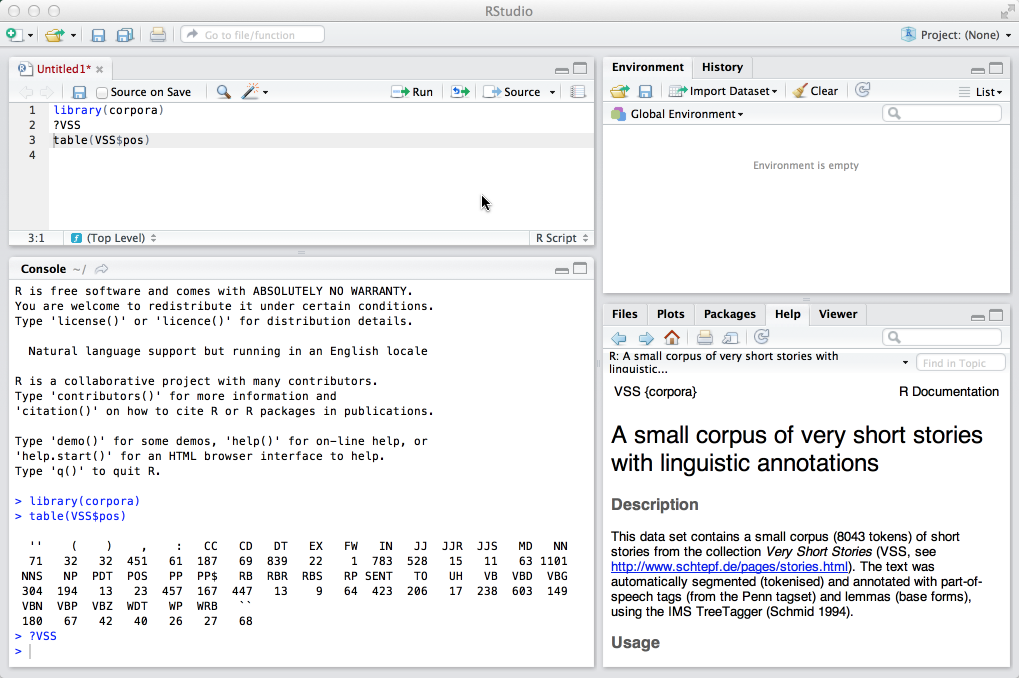
\includegraphics[width=10cm]{img/rstudio}

\end{frame}


%%%%%%%%%%%%%%%%%%%%%%%%%%%%%%%%%%%%%%%%%%
\subsection{Basic functionalities}

\begin{frame}[fragile]
  \frametitle{R as an oversized calculator}
  
\begin{alltt}
> 1+1  \begin{Rout}
[1] 2
\end{Rout}
> a <- 2     \REM{assignment does \emph{not} print anything by default}

> a * 2  \begin{Rout}
[1] 4
\end{Rout}
> log(a)     \REM{natural, i.e.\ base-\(e\) logarithm}\begin{Rout}
[1] 0.6931472
\end{Rout}
> log(a,2)   \REM{base-2 logarithm}\begin{Rout}
[1] 1
\end{Rout}
\end{alltt}

\end{frame}



\begin{frame}[fragile]
  \frametitle{Basic session management}
  \framesubtitle{Some of it is not necessary if you only use the GUI}

\ungap[1]
\begin{alltt}
\REM{to start R on command line, simply type ``\texttt{\textbf{R}}''}

setwd("path/to/data")  \REM{or use GUI menus}

ls()                   \REM{probably empty for now}

ls                     \REM{notice difference with previous line}

quit()                 \REM{or use GUI menus}
quit(save="yes")
quit(save="no")

\REM{NB: at least some interfaces support history recall, TAB completion, etc.}
\end{alltt}

\end{frame}


\begin{frame}[fragile]
  \frametitle{Vectorial math}

\ungap[1]
\begin{alltt}
> a <- c(1,2,3) \REM{\texttt{\textbf{c}} (for \emph{combine}) creates vectors}

> a * 2   \REM{operators are applied to each element of a vector}\begin{Rout}
[1] 2 4 6
\end{Rout}

> log(a)  \REM{also works for most standard functions}\begin{Rout}
[1] 0.0000000 0.6931472 1.0986123
\end{Rout}
> sum(a)  \REM{basic vector operations: sum, length, product, \ldots}\begin{Rout}
[1] 6
\end{Rout}
> length(a)\begin{Rout}
[1] 3
\end{Rout}
> sum(a)/length(a)\begin{Rout}
[1] 2
\end{Rout}
\end{alltt}

\end{frame}


\begin{frame}[fragile]
  \frametitle{Initializing vectors}

\begin{alltt}
> a <- 1:100            \REM{integer sequence}
> a

> a <- 10^(1:100)

> a <- seq(from=0, to=10, by=0.1) \REM{general sequence}

> a <- rnorm(100)       \REM{100 random numbers}

> a <- runif(100, 0, 5) \REM{what you're used to from Java etc.}
\end{alltt}
\end{frame}

\begin{frame}[fragile]
  \frametitle{Summary statistics}
  \framesubtitle{More about these summary statistics in Unit 3}

  \ungap[1]
\begin{alltt}
> length(a)

> summary(a)  \REM{statistical summary of numeric vector} \begin{Rout}
   Min. 1st Qu.  Median    Mean 3rd Qu.    Max. 
0.02717 0.51770 1.05200 1.74300 2.32600 9.11100  \end{Rout}

> mean(a)

> median(a)

> sd(a)       \REM{standard deviation is not included in summary}

> quantile(a) \begin{Rout}
    0%    25%    50%    75%   100% 
0.0272 0.5177 1.0518 2.3261 9.1107 \end{Rout}

> quantile(a,.75)
\end{alltt}

\end{frame}


\begin{frame}[fragile]
  \frametitle{Basic plotting}

  \ungap[1.5]
\begin{alltt}
> a <- 2^(1:100)        \REM{don't forget the parentheses!}
> plot(a)

> x <- 1:100            \REM{most often: plot \(x\) against \(y\)}
> y <- sqrt(x)
> plot(x, y)

> plot(x, a)
> plot(x, a, log="y")   \REM{various logarithmic plots}
> plot(x, a, log="x")
> plot(x, a, log="xy")
> plot(log(x), log(a))

> hist(rnorm(100))      \REM{histogram and density estimation}
> hist(rnorm(1000))
> plot(density(rnorm(100000)))
\end{alltt}

\end{frame}

\begin{frame}[fragile]
  \frametitle{(Slightly less) basic plotting}

  \ungap[1]
\begin{alltt}
> a <- rbinom(10000,100,.5)
> hist(a)

> hist(a, probability=TRUE)
> lines(density(a))

> hist(a, probability=TRUE)
> lines(density(a), col="red", lwd=3)

> hist(a, probability=TRUE, 
  main="Some Distribution", xlab="value",
  ylab="probability")  \REM{better to type command on a single line!}
> lines(density(a), col="red", lwd=3)
\end{alltt}

\end{frame}

\begin{frame}[fragile]
  \frametitle{Help!}

\begin{alltt}
> help("hist")  \REM{R has excellent online documentation}
> ?hist         \REM{short, convenient form of the help command} 

> help.search("histogram")

> ?help.search

> help.start()  \REM{searchable HTML documentation}

\REM{or use GUI menus to access \& search documentation}
\end{alltt}

\end{frame}



\begin{frame}[fragile]
  \frametitle{Your first R script}

  \begin{itemize}
  \item Simply type R commands into a text file \& save it
  \item Use built-in GUI functionality or external text editor
    \begin{itemize}
    \item Microsoft Word is \emph{not} a text editor!
    \item nor is Apple's TextEdit application \ldots
    \item[]
    \end{itemize}
  \item Execute R script from GUI editor or by typing
    \begin{alltt}
> source("my_script.R") \REM{more about files later}
> source(file.choose()) \REM{select with file dialog box}
    \end{alltt}
  \item Many GUI editors can execute scripts line by line
    \begin{itemize}
    \item check your editor's documentation for keyboard shortcuts
    \item[]
    \end{itemize}
  \item Just typing an expression will not automatically print the result in a
    script: use \verb_print(sd(a))_ instead of \verb_sd(a)_
  \end{itemize}
\end{frame}

%%%%%%%%%%%%%%%%%%%%%%%%%%%%%%%%%%%%%%%%%%
\subsection{External files and data-frames}

{
\newcommand{\tri}{{\color{secondary!60!white}\scriptsize $\,^{\blacktriangleright}$}}
\begin{frame}[fragile]
  \frametitle{Input from an external file}

  \begin{itemize}
  \item We like to keep our data in space- or TAB-delimited text files with a
    first row (``header'') labeling the fields:
\begin{alltt}
word\tri frequency\tri cat
dog\tri  15\tri        noun
bark\tri 10\tri        verb 
\end{alltt}
  \item This is an easy format to import into R, and it is easy to
    convert to/from other tabular formats using standard tools
  \item We assume that external input is always in this format\\ (or can
    easily be converted to it)
    \begin{itemize}
    \item spreadsheet applications prefer CSV (comma-separated values),
      which R also reads and writes quite well
    \item Microsoft Excel is a nice table editor, but beware of localised
      number formats
    \end{itemize}
  \end{itemize}

\end{frame}
}


\begin{frame}[fragile]
  \frametitle{Reading a TAB-delimited file with header}
  
\begin{alltt}
> brown <- read.table("brown.stats.txt",
  header=TRUE)
\REM{if file is not in working directory, you must specify the full path}
\REM{(or use \texttt{setwd()} function we introduced before)}

\REM{exact behaviour of \texttt{file.choose()} depends on operating system}
> brown <- read.table(file.choose(), header=TRUE)

\REM{more robust if you are sure file is in tab-delimited format}
> brown <- read.delim("brown.stats.txt")

\REM{this data set is also included in the SIGIL package}
> library(SIGIL)
> brown <- BrownStats
\end{alltt}

\end{frame}


\begin{frame}[fragile]
  \frametitle{Reading and writing CSV files}
  
  \ungap[1.5]
\begin{alltt}
\REM{R can also read and write files in CSV format}
> write.csv(brown, "brown.stats.csv",
  row.names=FALSE)
\REM{this is convenient for exchanging data with database and}
\REM{spreadsheet software (or using Excel as a data editor)}

\REM{NB: comma-separated values are not always separated by commas}
\REM{(e.g.\ in German; use \texttt{write.csv2} if Excel doesn't recognise columns)}
> write.csv2(brown, "brown.stats.csv",
  row.names=FALSE)

\REM{TASK: load \texttt{brown.stats.csv} into Excel or OpenOffice.org}

\REM{check generated CSV file (use \texttt{read.csv2} with \texttt{write.csv2} above)}
> brown.csv <- read.csv("brown.stats.csv")
> all.equal(brown.csv, brown)
\end{alltt}

\end{frame}


\begin{frame}
  \frametitle{Data frames}

  \begin{itemize}
  \item The commands above create a \h{data frame}
  \item This is the basic data structure (object)\\
    used to represent statistical tables in R
    \begin{itemize}
    \item rows = objects or ``observations''
    \item columns = variables, i.e.\ measured quantities
    \item[]
    \end{itemize}
  \item Different types of variables
    \begin{itemize}
    \item numerical variables (what we've used so far)
    \item Boolean variables
    \item factor variables (nominal or ordinal classification)
    \item string variables
    \item[]
    \end{itemize}
  \item Technically, data frames are collections of column vectors\\
    (of the same length), and we will think of them as such
  \end{itemize}

\end{frame}


\begin{frame}[fragile]
  \frametitle{Data frames}

\begin{alltt}
> summary(brown)

> colnames(brown)

> dim(brown)       \REM{number of rows and columns}

> head(brown)

> plot(brown)
\end{alltt}

\end{frame}


\begin{frame}
  \frametitle{Type/token counts and word lengths for Brown \& LOB texts}

  Data files in TAB-delimited format:
  \begin{itemize}
  \item \url{brown.stats.txt}: information for Brown corpus (AmE)
  \item \url{lob.stats.txt}: information for LOB corpus (BrE)
  \end{itemize}

  \gap
  Variables:
  \begin{description}
  \item[to] Token count
  \item[ty] Type count (\emph{distinct} words)
  \item[se] Sentence count
  \item[towl] Average word length\\ (averaged across tokens in document)
  \item[tywl] Average word length\\ (averaged across distinct types in
    document)
  \end{description}
\end{frame}


\begin{frame}[fragile]
  \frametitle{Access vectors inside a data frame}

\ungap[1]
\begin{alltt}
> brown$to
> head(brown$to)

\REM{TASK: compute summary statistics (length, mean, max, etc.)}
\REM{for vectors in the Brown data frame}

\REM{what does the following do?}
> summary(brown$ty / brown$to)

> attach(brown)   \REM{attach data frame for convenient access}
> summary(ty/to)
> detach()        \REM{detach from search path}

> with(brown, summary(ty/to)) \REM{a better approach}
\end{alltt}

\end{frame}

\begin{frame}[fragile]
  \frametitle{More data access}

\begin{alltt}
> brown$ty[1]    \REM{vector indexing starts with 1}
> brown[1,2]     \REM{row, column}

> brown$ty[1:10] \REM{use arbitrary vectors as indices}
> brown[1:10,2]

> brown[1,]
> brown[,2]
\end{alltt}

\end{frame}


\begin{frame}[fragile]
  \frametitle{Conditional selection}


\begin{alltt}
> brown[brown$to < 2200, ]  \REM{index with Boolean vector}
> brown$ty[brown$to >= 2200]
> sum(brown$to >= 2200)     \REM{standard way to count matches}

> subset(brown, to < 2200)  \REM{syntactic sugar (similar to \texttt{with})}
> lessdata <- subset(brown, to < 2200)

> a <- brown$ty[brown$to >= 2200]

\REM{equality: == (also works for strings)}
\REM{inequality: !=}
\REM{complex constraints: and &, or |, not !}
\REM{NB: always use single characters, not && or ||}
\end{alltt}

\end{frame}

%%%%%%%%%%%%%%%%%%%%%%%%%%%%%%%%%%%%%%%%%%
\subsection{A simple case study: comparing Brown and LOB}

\begin{frame}
  \frametitle{Procedure}
  \framesubtitle{The methods used here will be explained in Units 3 and 6}

    \begin{itemize}
    \item Collect basic summary statistics for the two corpora
    \item Check if there is a significant difference in the token counts
      (since document length was controlled by corpus builders)
    \item If difference is significant (we will see that it is), then
      type counts are not directly comparable, and sentence
      counts should be normalized (divide by token count)
    \item Is word length correlated to document length?\\
      (corpus comparison would also not be appropriate in this case)%
      \pause
    \item Please read the LOB data set into a data frame named \texttt{lob}
      now, and take a look at its basic statistics
      \begin{itemize}
      \item file \texttt{lob.stats.txt}, or \texttt{LOBStats} in \texttt{SIGIL} package
      \end{itemize}
    \item Also, plot the data frame for a first impression of correlations
      between the variables
    \end{itemize}

\end{frame}

\begin{frame}[fragile]
  \frametitle{Comparing token counts}

\ungap[1]
\begin{alltt}
> boxplot(brown$to,lob$to)
> boxplot(brown$to,lob$to,names=c("brown","lob"))
> boxplot(brown$to,lob$to,names=c("brown","lob"),
  ylim=c(1500,3000))
> ?boxplot

> t.test(brown$to, lob$to)
> wilcox.test(brown$to, lob$to)

> brown.to.center <- 
  with(brown, to[to > 2200 & to < 2400])
> lob.to.center <- 
  with(lob, to[to > 2200 & to < 2400])

> t.test(brown.to.center, lob.to.center)

\REM{how about sentence length?}
\end{alltt}

\end{frame}

\begin{frame}[fragile]
  \frametitle{Is word length correlated with token count?}

\begin{alltt}
\REM{average word length by tokens and types is almost the same:}

> plot(brown$towl, brown$tywl)
> cor.test(brown$towl, brown$tywl)
> cor.test(brown$towl, brown$tywl, method="spearman")

\REM{correlation with token count}

> plot(brown$to, brown$towl)
> cor.test(brown$to, brown$towl)
\end{alltt}

\end{frame}

%%%%%%%%%%%%%%%%%%%%%%%%%%%%%%%%%%%%%%%%%%%%%%%%%%%%%%%%%%%%%%%%%%%%%%
%% References (if any)

%% \frame[allowframebreaks]{
%%   \frametitle{References}
%%   \bibliographystyle{natbib-stefan}
%%   \begin{scriptsize}
%%     \bibliography{sigil}
%%   \end{scriptsize}
%% }

\end{document}
